% \textbf{\underline{OZ 6 - Magnetische inductie en de wet van Faraday - Oefening 1:}}
% \vspace{0.5cm}

% Een geleidende staaf van lengte $ l = 35,0 $ cm kan wrijvingsloos bewegen op twee parallelle geleidende rails zoals aangegeven in Figuur 6.1. Twee weerstanden $ R_1 = 2,00 \ \Omega $ en $ R_2 = 5,00 \ \Omega $ zijn verbonden met de uiteinden van de twee rails. Een constant magneetveld $ B = 2,50 $ T staat loodrecht op het vlak van de rails en is in het blad gericht. Men trekt nu de staaf naar links met een constante snelheid $ v = 8,00 $ m/s.

% \begin{enumerate}[(a)]
%     \item Bepaal de stromen door de twee weerstanden.
%     \item Bereken het totale vermogen dat gedissipeerd wordt door de weerstanden in het circuit.
%     \item Bepaal de grootte en richting van de kracht die men moet uitoefenen op de staaf.
%     \item Wat is het mechanisch vermogen dat men moet uitoefen om de staaf te bewegen.
% \end{enumerate}

% \begin{figure}[H]
%     \centering
%     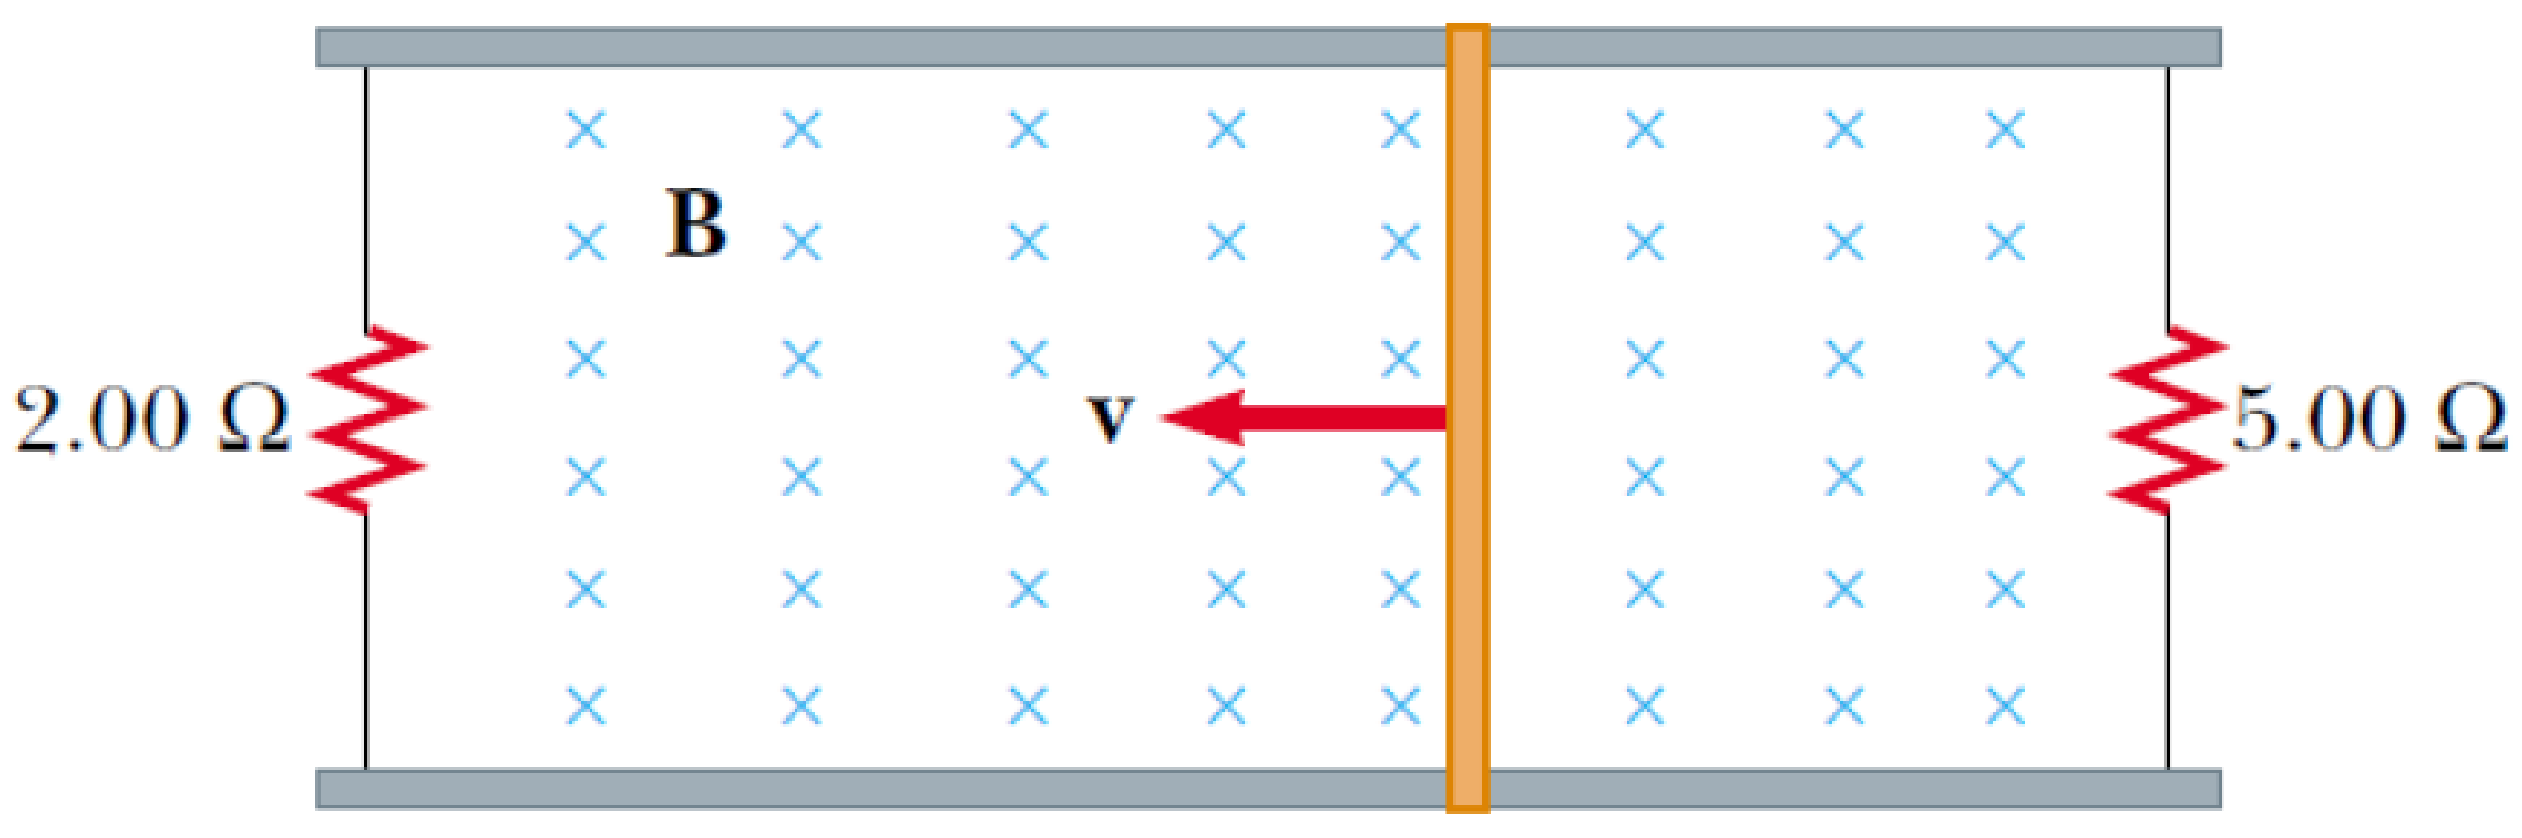
\includegraphics[width=9cm]{oz06/resources/oef-1-opgave.png}
    
%     \textbf{Figuur 6.1}
% \end{figure}

% \begin{description}[labelwidth=1.5cm, leftmargin=!]
%     \item[Geg. :]   $ l = 35,0 $ cm; $ R_1 = 2,00 \ \Omega $; $ R_2 = 5,00 \ \Omega $; $ B = 2,50 $ T; $ v = 8,00 $ m/s;
% \end{description}

% \begin{figure}[H]
%     \centering
%     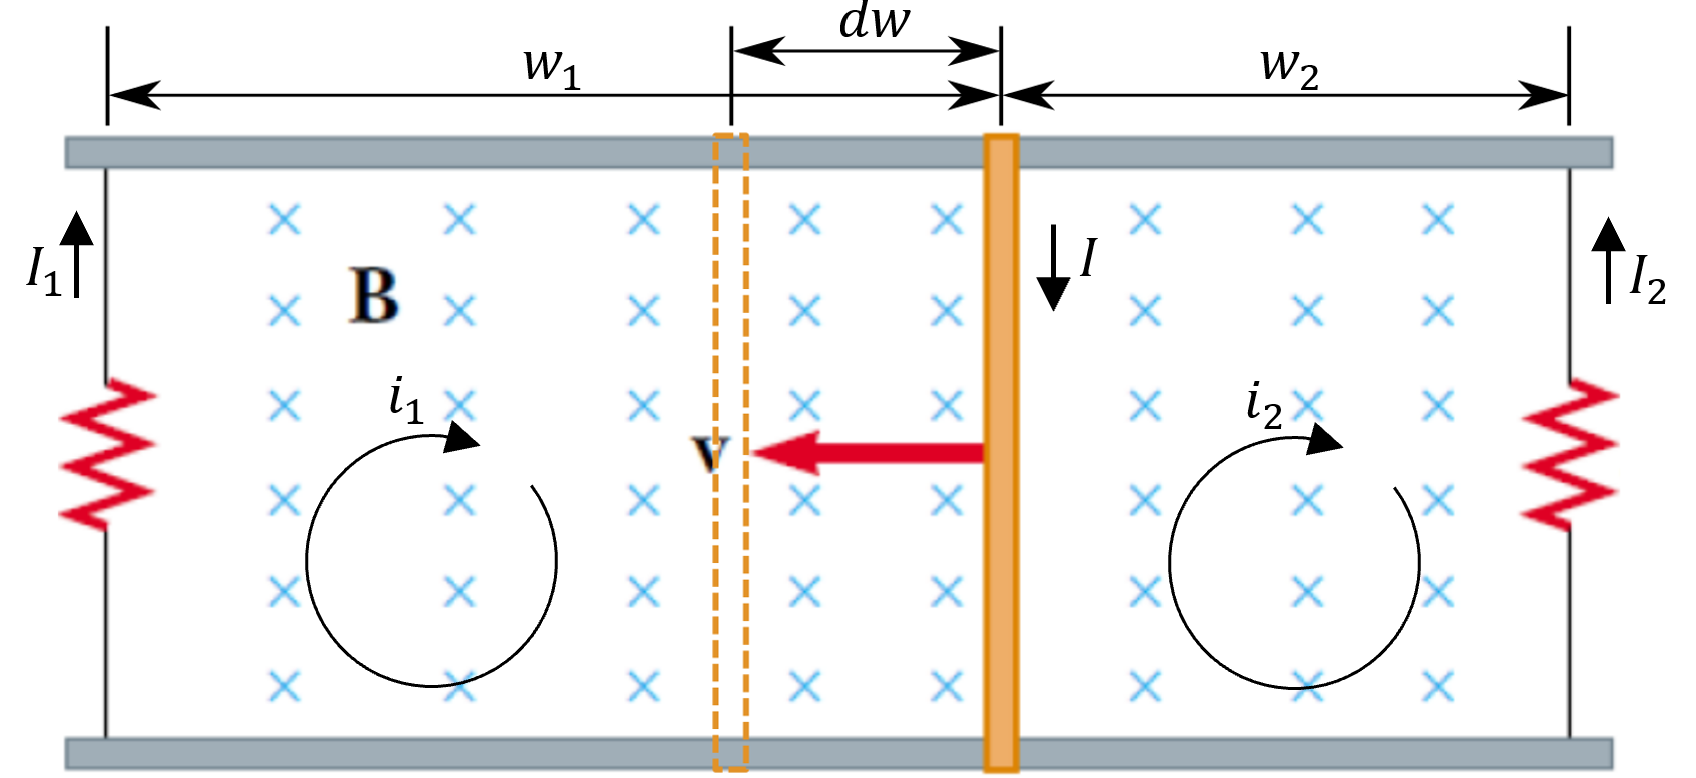
\includegraphics[width=7cm]{oz06/resources/oef-1-schets.png}
    
%     \textbf{Schets 6.1}
% \end{figure}

% \begin{enumerate}[(a)]
%     \item 
%         \begin{description}[labelwidth=1.5cm, leftmargin=!]
%             \item[Gevr. :]  $ I_1 $; $ I_2 $;
%             \item[Opl. :]   $ A_1 = l \cdot \left( w_1 - dw \right) = l \cdot \left( w_1 - v t \right) $
            
%                             $ \Phi_1 = \int{ \vec{B} \cdot d\vec{A_1}} 
%                             = B \cdot A_1 
%                             = B \cdot l \cdot \left( w_1 - v t \right) $
                            
%                             \hspace{-0.57cm} $ \Rightarrow 
%                             \dfrac{d\Phi_1}{dt} = -B \cdot l \cdot v $
                            
%                             $ \varepsilon_1 = -\dfrac{d\Phi_1}{dt} = B \cdot l \cdot v $
                            
%                             $ i_1 = \dfrac{\varepsilon_1}{R_1} = \dfrac{B \cdot l \cdot v}{R_1} = \dfrac{2,50 \cdot 35,0 \cdot 10^{-2} \cdot 8,00}{2,00} = 3,50 $ A
                            
%                             $ I_1 = i_3 = 3,50 $ A
                            
%                             \vspace{0.5cm}
                            
%                             $ A_2 = l \cdot \left( w_2 + dw \right) = l \cdot \left( w_2 + v t \right) $
            
%                             $ \Phi_2 = \int{ \vec{B} \cdot d\vec{A_2}} 
%                             = B \cdot A_2 
%                             = B \cdot l \cdot \left( w_2 + v t \right) $
                            
%                             \hspace{-0.57cm} $ \Rightarrow 
%                             \dfrac{d\Phi_2}{dt} = B \cdot l \cdot v $
                            
%                             $ \varepsilon_2 = -\dfrac{d\Phi_2}{dt} = -B \cdot l \cdot v $
                            
%                             $ i_2 = \dfrac{\varepsilon_2}{R_2} = \dfrac{-B \cdot l \cdot v}{R_2} = \dfrac{2,50 \cdot 35,0 \cdot 10^{-2} \cdot 8,00}{5,00} = -1,40 $ A
                            
%                             $ I_2 = -i_2 = 1,40 $ A
%         \end{description}
%     \item
%         \begin{description}[labelwidth=1.5cm, leftmargin=!]
%             \item[Gevr. :]  $ P $;
%             \item[Opl. :]   $ P_1 = I_1^2 \cdot R_1 = 3,50^2 \cdot 2,00 = 24,5 $ W
            
%                             $ P_2 = I_2^2 \cdot R^2 = (-1,40)^2 \cdot 5,00 = 9,8 W $
                            
%                             $ P = P_1 + P_2 = 24,5 + 9,8 = 34,3 $ W
%         \end{description}
%     \item
%         \begin{description}[labelwidth=1.5cm, leftmargin=!]
%             \item[Gevr. :]  $ F $;
%             \item[Opl. :]   $ I = I_1 + I_2 = 3,50 + 1,40 = 4,90 $ A
                            
%                             $ d\vec{F} = I d\vec{s} \times \vec{B} $
                            
%                             \hspace{-0.57cm} $ \Rightarrow
%                             F = I ds B \cdot \cos{0^{\circ}} 
%                             = I B ds $
                            
%                             $ \int_{0}^{F}{dF} = \int_{0}^{l}{I B ds} $
                            
%                             $ F = I B l = 4,90 \cdot 2,50 \cdot 35,0 \cdot 10^{-2} = 4,2875 $ N $ 
%                             \approx 4,29 $ N
%         \end{description}
%     \item
%         \begin{description}[labelwidth=1.5cm, leftmargin=!]
%             \item[Gevr. :]  $ P_m $;
%             \item[Opl. :]   $ dW = \vec{F} \cdot d\vec{r} = F \cdot dr = F \cdot v \cdot dt $
            
%                             $ P_m = \dfrac{dW}{dt} = F \cdot v = 4,2875 \cdot 8,00 = 34,3 $ W
%         \end{description}
% \end{enumerate}

% \vspace{1cm}